\documentclass{article}
\usepackage[utf8]{inputenc}

\usepackage[paperwidth=8.5in, paperheight=11in, top=1in, bottom=.5in, left=.5in, right=.5in]{geometry}
\usepackage{fancyhdr, graphicx,tikz,amsmath,multicol,paracol,pgfplots}
\usepackage[inline]{enumitem}

\pagestyle{fancy}
\lhead{\large{\textbf{Module 8: Trigonometric Equations (TE) - Readiness Assurance Test}}}
\chead{}
\rhead{}
\lfoot{}
\cfoot{}
%\rfoot{\thepage/\pageref{LastPage} }
\setlength{\headheight}{14pt} %added in bc warning

%%% LIST ANSWER KEY HERE

% 1 B
% 2 B
% 3 C
% 4 A
% 5 B
% 6 D
% 7 A
% 8 A
% 9 D
% 10 C


\begin{document}


\begin{enumerate}

% Determine quadrant of trigonometric functions.

\item Which trigonometric function is positive in Quadrant III?

  \begin{enumerate}
  \begin{multicols}{4}
  \item cosine 
  \item tangent %Correct
  \item secant
  \item sine 
  \end{multicols}
  \end{enumerate}
  
\item Let $\theta$ be an angle in standard position. In which quadrant does $\theta$ lie if $\sin\theta>0$ and $\sec\theta<0$?

  \begin{enumerate}
  \begin{multicols}{4}
  \item Quadrant I  
  \item Quadrant II %correct 
  \item Quadrant III
  \item Quadrant IV
  \end{multicols}
  \end{enumerate}

% Reciprocal functions and trig relationships.

\item Cosecant is the reciprocal of which function?

  \begin{enumerate}
  \begin{multicols}{4}
  \item secant  
  \item cosine 
  \item sine %correct 
  \item tangent
  \end{multicols}
  \end{enumerate}

\item Let $\theta$ be an angle in standard position in Quadrant I. Suppose that $\sin\theta=\frac{4}{5}$. What is the value of $\sec\theta$?

  \begin{enumerate}
  \begin{multicols}{4}
  \item $\frac{5}{3}$ %correct 
  \item $-\frac{4}{5}$ 
  \item $\frac{3}{5}$  
  \item $\frac{3}{5}$
  \end{multicols}
  \end{enumerate}

%Solve a linear equation.

\item Solve for $w$ in the equation: $4(-2w+9)=-2(3w-7)$

  \begin{enumerate}
  \begin{multicols}{4}
  \item $w=-11$  
  \item $w=11$ %correct
  \item $w=10$  
  \item $w=12$
  \end{multicols}
  \end{enumerate}
  
%Determine trigonometric ratios.

\vspace{5pt}
\hspace{-15pt}\textbf{Use the right triangle $ABC$, as shown in the figure below, to answer questions 6-7.}

\begin{center}
    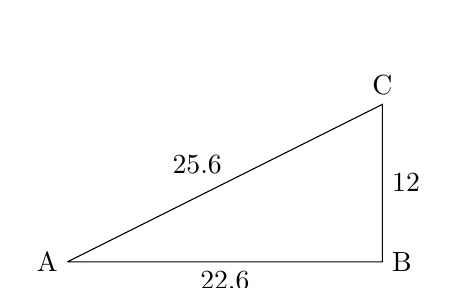
\begin{tikzpicture}
        \coordinate (a) at (0,0);
        \coordinate (b) at (4,0);
        \coordinate (c) at (4,2);
        \draw (a) -- (b)node[midway, below]{22.6} -- (c)node[midway,right]{12} -- (a)node[midway,left={1em}, above]{25.6}; % Triangle.

        \draw (a) node[anchor=east,align=center] {A};
        \draw (b) node[anchor=west,align=center] {B};
        \draw (c) node[anchor=south]{C};
    \end{tikzpicture}
    \end{center}

\item What is the tangent ratio for angle $C$?

  \begin{enumerate}
  \begin{multicols}{4}
  \item $\frac{12}{22.6}$  
  \item $\frac{22.6}{25.6}$
  \item $\frac{25.6}{22.6}$ 
  \item $\frac{22.6}{12}$ %correct
  \end{multicols}
  \end{enumerate}

\item What is the sine ratio for angle $A$?

  \begin{enumerate}
  \begin{multicols}{4}
  \item $\frac{12}{25.6}$ %correct 
  \item $\frac{22.6}{12}$
  \item $\frac{12}{22.6}$ 
  \item $\frac{25.6}{12}$ 
  \end{multicols}
  \end{enumerate}

% Solve quadratic equations (with and without factoring).
\vspace{5pt}
\hspace{-15pt}\textbf{For questions 8-10, solve each quadratic equation.}

\item $(2m-1)^2=49$

  \begin{enumerate}
  \begin{multicols}{4}
  \item $m=4, -3$  %correct
  \item $m=3, -4$
  \item $m=6, -8$  
  \item $m=8, -6$
  \end{multicols}
  \end{enumerate}
  
\item $x^2+13x=-40$

  \begin{enumerate}
  \begin{multicols}{4}
  \item $x=-8, 5$  
  \item $x=-40, -1$
  \item $x=5, 8$  
  \item $x=-8, -5$ %correct
  \end{multicols}
  \end{enumerate}

\item $12y^2+15=-29y$

  \begin{enumerate}
  \begin{multicols}{4}
  \item $y=\frac{5}{3}, -\frac{3}{4}$  
  \item $y=-\frac{5}{12}, -\frac{1}{5}$
  \item $y=-\frac{5}{3}, -\frac{3}{4}$  %correct
  \item $y=\frac{5}{3}, \frac{3}{4}$
  \end{multicols}
  \end{enumerate}


\end{enumerate}


\end{document}